\documentclass[1p]{elsarticle_modified}
%\bibliographystyle{elsarticle-num}

%\usepackage[colorlinks]{hyperref}
%\usepackage{abbrmath_seonhwa} %\Abb, \Ascr, \Acal ,\Abf, \Afrak
\usepackage{amsfonts}
\usepackage{amssymb}
\usepackage{amsmath}
\usepackage{amsthm}
\usepackage{scalefnt}
\usepackage{amsbsy}
\usepackage{kotex}
\usepackage{caption}
\usepackage{subfig}
\usepackage{color}
\usepackage{graphicx}
\usepackage{xcolor} %% white, black, red, green, blue, cyan, magenta, yellow
\usepackage{float}
\usepackage{setspace}
\usepackage{hyperref}

\usepackage{tikz}
\usetikzlibrary{arrows}

\usepackage{multirow}
\usepackage{array} % fixed length table
\usepackage{hhline}

%%%%%%%%%%%%%%%%%%%%%
\makeatletter
\renewcommand*\env@matrix[1][\arraystretch]{%
	\edef\arraystretch{#1}%
	\hskip -\arraycolsep
	\let\@ifnextchar\new@ifnextchar
	\array{*\c@MaxMatrixCols c}}
\makeatother %https://tex.stackexchange.com/questions/14071/how-can-i-increase-the-line-spacing-in-a-matrix
%%%%%%%%%%%%%%%

\usepackage[normalem]{ulem}

\newcommand{\msout}[1]{\ifmmode\text{\sout{\ensuremath{#1}}}\else\sout{#1}\fi}
%SOURCE: \msout is \stkout macro in https://tex.stackexchange.com/questions/20609/strikeout-in-math-mode

\newcommand{\cancel}[1]{
	\ifmmode
	{\color{red}\msout{#1}}
	\else
	{\color{red}\sout{#1}}
	\fi
}

\newcommand{\add}[1]{
	{\color{blue}\uwave{#1}}
}

\newcommand{\replace}[2]{
	\ifmmode
	{\color{red}\msout{#1}}{\color{blue}\uwave{#2}}
	\else
	{\color{red}\sout{#1}}{\color{blue}\uwave{#2}}
	\fi
}

\newcommand{\Sol}{\mathcal{S}} %segment
\newcommand{\D}{D} %diagram
\newcommand{\A}{\mathcal{A}} %arc


%%%%%%%%%%%%%%%%%%%%%%%%%%%%%5 test

\def\sl{\operatorname{\textup{SL}}(2,\Cbb)}
\def\psl{\operatorname{\textup{PSL}}(2,\Cbb)}
\def\quan{\mkern 1mu \triangleright \mkern 1mu}

\theoremstyle{definition}
\newtheorem{thm}{Theorem}[section]
\newtheorem{prop}[thm]{Proposition}
\newtheorem{lem}[thm]{Lemma}
\newtheorem{ques}[thm]{Question}
\newtheorem{cor}[thm]{Corollary}
\newtheorem{defn}[thm]{Definition}
\newtheorem{exam}[thm]{Example}
\newtheorem{rmk}[thm]{Remark}
\newtheorem{alg}[thm]{Algorithm}

\newcommand{\I}{\sqrt{-1}}
\begin{document}

%\begin{frontmatter}
%
%\title{Boundary parabolic representations of knots up to 8 crossings}
%
%%% Group authors per affiliation:
%\author{Yunhi Cho} 
%\address{Department of Mathematics, University of Seoul, Seoul, Korea}
%\ead{yhcho@uos.ac.kr}
%
%
%\author{Seonhwa Kim} %\fnref{s_kim}}
%\address{Center for Geometry and Physics, Institute for Basic Science, Pohang, 37673, Korea}
%\ead{ryeona17@ibs.re.kr}
%
%\author{Hyuk Kim}
%\address{Department of Mathematical Sciences, Seoul National University, Seoul 08826, Korea}
%\ead{hyukkim@snu.ac.kr}
%
%\author{Seokbeom Yoon}
%\address{Department of Mathematical Sciences, Seoul National University, Seoul, 08826,  Korea}
%\ead{sbyoon15@snu.ac.kr}
%
%\begin{abstract}
%We find all boundary parabolic representation of knots up to 8 crossings.
%
%\end{abstract}
%\begin{keyword}
%    \MSC[2010] 57M25 
%\end{keyword}
%
%\end{frontmatter}

%\linenumbers
%\tableofcontents
%
\newcommand\colored[1]{\textcolor{white}{\rule[-0.35ex]{0.8em}{1.4ex}}\kern-0.8em\color{red} #1}%
%\newcommand\colored[1]{\textcolor{white}{ #1}\kern-2.17ex	\textcolor{white}{ #1}\kern-1.81ex	\textcolor{white}{ #1}\kern-2.15ex\color{red}#1	}

{\Large $\underline{12n_{0517}~(K12n_{0517})}$}

\setlength{\tabcolsep}{10pt}
\renewcommand{\arraystretch}{1.6}
\vspace{1cm}\begin{tabular}{m{100pt}>{\centering\arraybackslash}m{274pt}}
\multirow{5}{120pt}{
	\centering
	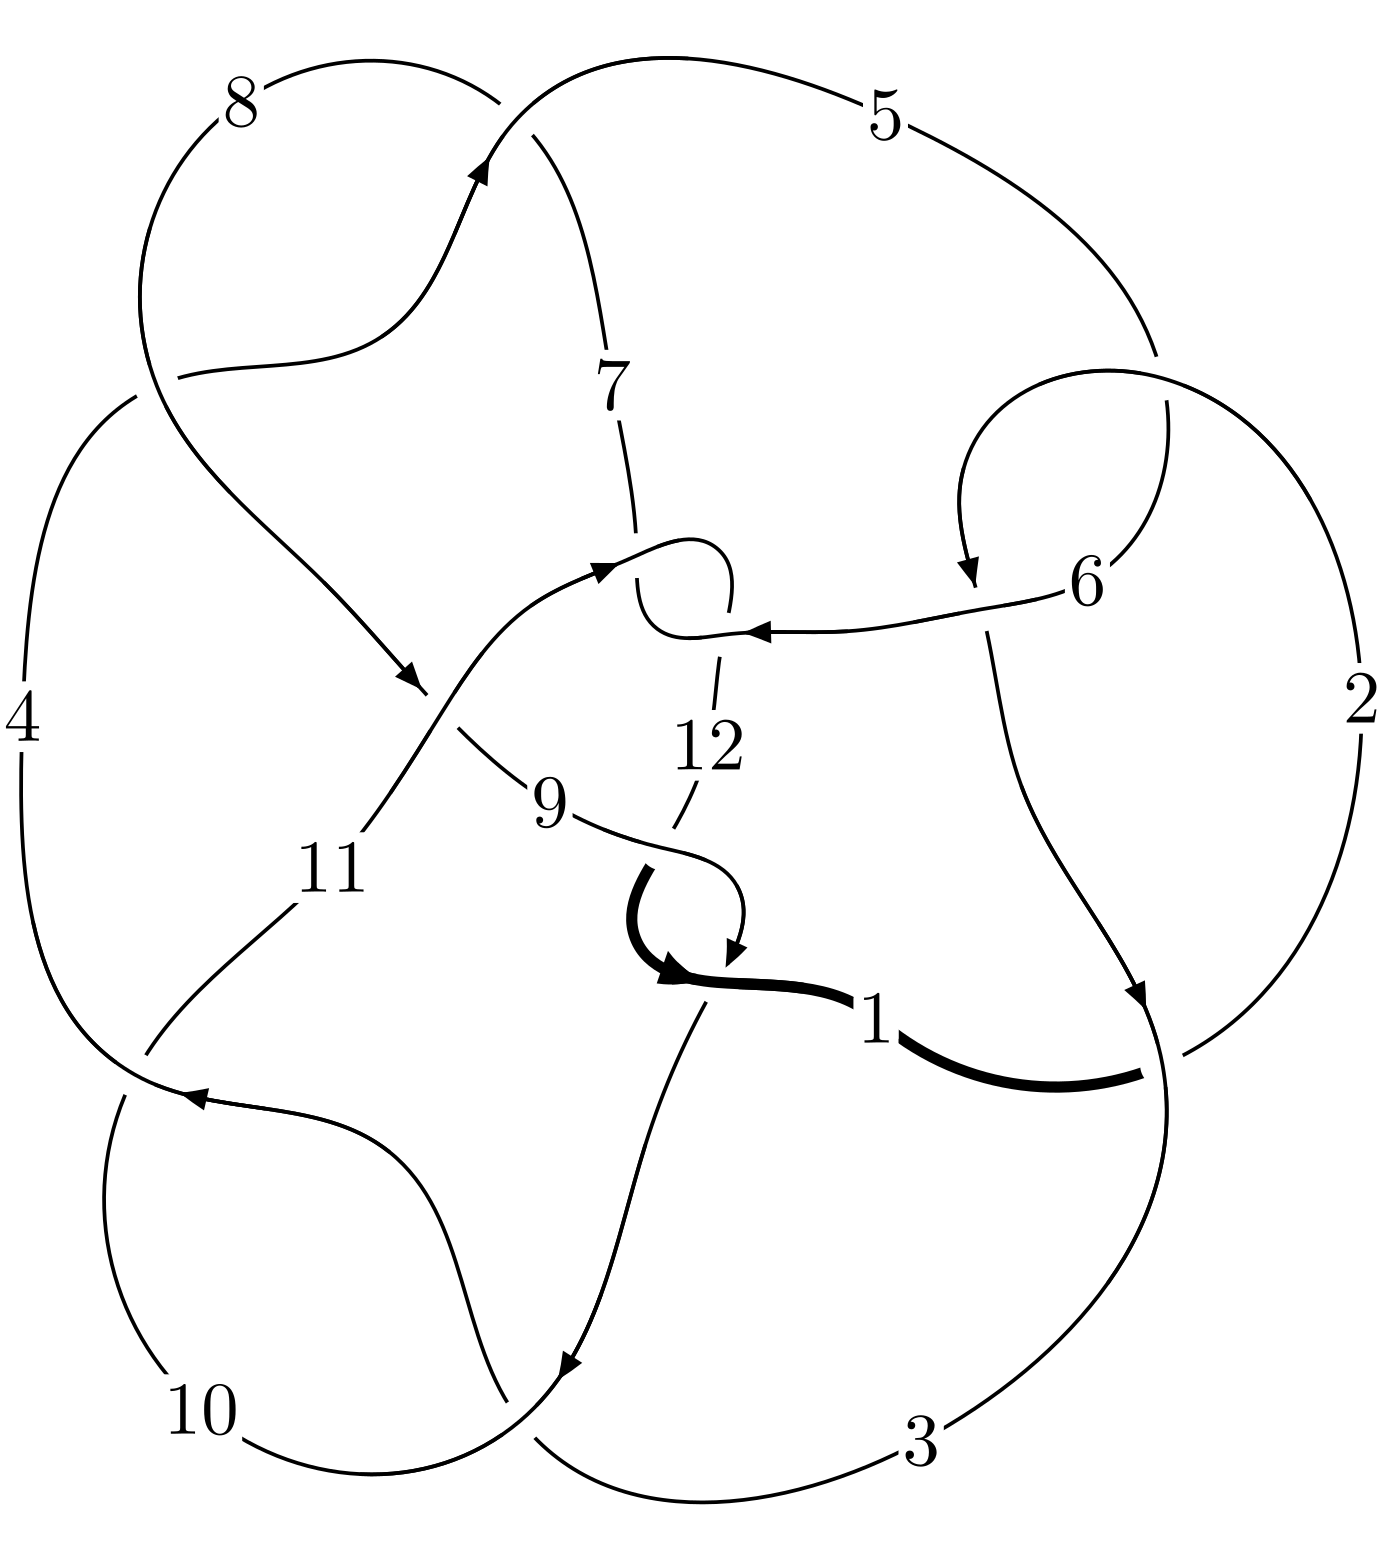
\includegraphics[width=112pt]{../../../GIT/diagram.site/Diagrams/png/2606_12n_0517.png}\\
\ \ \ A knot diagram\footnotemark}&
\allowdisplaybreaks
\textbf{Linearized knot diagam} \\
\cline{2-2}
 &
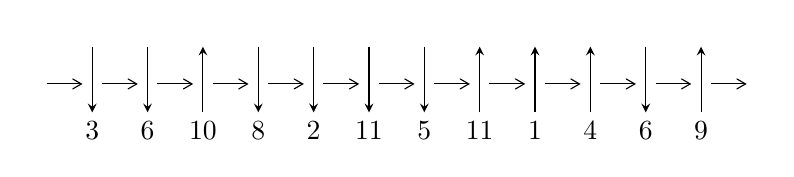
\begin{tikzpicture}[x=20pt, y=17pt]
	% nodes
	\node (C0) at (0, 0) {};
	\node (C1) at (1, 0) {};
	\node (C1U) at (1, +1) {};
	\node (C1D) at (1, -1) {3};

	\node (C2) at (2, 0) {};
	\node (C2U) at (2, +1) {};
	\node (C2D) at (2, -1) {6};

	\node (C3) at (3, 0) {};
	\node (C3U) at (3, +1) {};
	\node (C3D) at (3, -1) {10};

	\node (C4) at (4, 0) {};
	\node (C4U) at (4, +1) {};
	\node (C4D) at (4, -1) {8};

	\node (C5) at (5, 0) {};
	\node (C5U) at (5, +1) {};
	\node (C5D) at (5, -1) {2};

	\node (C6) at (6, 0) {};
	\node (C6U) at (6, +1) {};
	\node (C6D) at (6, -1) {11};

	\node (C7) at (7, 0) {};
	\node (C7U) at (7, +1) {};
	\node (C7D) at (7, -1) {5};

	\node (C8) at (8, 0) {};
	\node (C8U) at (8, +1) {};
	\node (C8D) at (8, -1) {11};

	\node (C9) at (9, 0) {};
	\node (C9U) at (9, +1) {};
	\node (C9D) at (9, -1) {1};

	\node (C10) at (10, 0) {};
	\node (C10U) at (10, +1) {};
	\node (C10D) at (10, -1) {4};

	\node (C11) at (11, 0) {};
	\node (C11U) at (11, +1) {};
	\node (C11D) at (11, -1) {6};

	\node (C12) at (12, 0) {};
	\node (C12U) at (12, +1) {};
	\node (C12D) at (12, -1) {9};
	\node (C13) at (13, 0) {};

	% arrows
	\draw[->,>={angle 60}]
	(C0) edge (C1) (C1) edge (C2) (C2) edge (C3) (C3) edge (C4) (C4) edge (C5) (C5) edge (C6) (C6) edge (C7) (C7) edge (C8) (C8) edge (C9) (C9) edge (C10) (C10) edge (C11) (C11) edge (C12) (C12) edge (C13) ;	\draw[->,>=stealth]
	(C1U) edge (C1D) (C2U) edge (C2D) (C3D) edge (C3U) (C4U) edge (C4D) (C5U) edge (C5D) (C6U) edge (C6D) (C7U) edge (C7D) (C8D) edge (C8U) (C9D) edge (C9U) (C10D) edge (C10U) (C11U) edge (C11D) (C12D) edge (C12U) ;
	\end{tikzpicture} \\
\hhline{~~} \\& 
\textbf{Solving Sequence} \\ \cline{2-2} 
 &
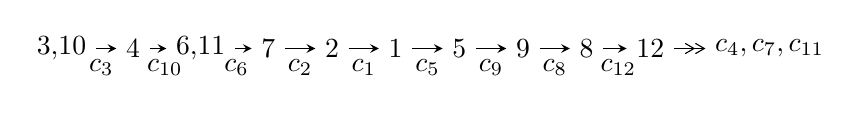
\begin{tikzpicture}[x=23pt, y=7pt]
	% node
	\node (A0) at (-1/8, 0) {3,10};
	\node (A1) at (1, 0) {4};
	\node (A2) at (33/16, 0) {6,11};
	\node (A3) at (25/8, 0) {7};
	\node (A4) at (33/8, 0) {2};
	\node (A5) at (41/8, 0) {1};
	\node (A6) at (49/8, 0) {5};
	\node (A7) at (57/8, 0) {9};
	\node (A8) at (65/8, 0) {8};
	\node (A9) at (73/8, 0) {12};
	\node (C1) at (1/2, -1) {$c_{3}$};
	\node (C2) at (3/2, -1) {$c_{10}$};
	\node (C3) at (21/8, -1) {$c_{6}$};
	\node (C4) at (29/8, -1) {$c_{2}$};
	\node (C5) at (37/8, -1) {$c_{1}$};
	\node (C6) at (45/8, -1) {$c_{5}$};
	\node (C7) at (53/8, -1) {$c_{9}$};
	\node (C8) at (61/8, -1) {$c_{8}$};
	\node (C9) at (69/8, -1) {$c_{12}$};
	\node (A10) at (11, 0) {$c_{4},c_{7},c_{11}$};

	% edge
	\draw[->,>=stealth]	
	(A0) edge (A1) (A1) edge (A2) (A2) edge (A3) (A3) edge (A4) (A4) edge (A5) (A5) edge (A6) (A6) edge (A7) (A7) edge (A8) (A8) edge (A9) ;
	\draw[->>,>={angle 60}]	
	(A9) edge (A10);
\end{tikzpicture} \\ 

\end{tabular} \\

\footnotetext{
The image of knot diagram is generated by the software ``\textbf{Draw programme}" developed by Andrew Bartholomew(\url{http://www.layer8.co.uk/maths/draw/index.htm\#Running-draw}), where we modified some parts for our purpose(\url{https://github.com/CATsTAILs/LinksPainter}).
}\phantom \\ \newline 
\centering \textbf{Ideals for irreducible components\footnotemark of $X_{\text{par}}$} 
 
\begin{align*}
I^u_{1}&=\langle 
2.59090\times10^{123} u^{69}-1.74742\times10^{122} u^{68}+\cdots+5.02254\times10^{123} b+2.90544\times10^{125},\\
\phantom{I^u_{1}}&\phantom{= \langle  }-2.56644\times10^{125} u^{69}+1.38382\times10^{124} u^{68}+\cdots+1.19537\times10^{125} a-2.88247\times10^{127},\\
\phantom{I^u_{1}}&\phantom{= \langle  }u^{70}+u^{69}+\cdots+167 u+119\rangle \\
I^u_{2}&=\langle 
u^{19}-11 u^{17}+\cdots+b+4 u,\;- u^{17}+10 u^{15}+\cdots+a-1,\;u^{20}-12 u^{18}+\cdots-4 u+1\rangle \\
\\
\end{align*}
\raggedright * 2 irreducible components of $\dim_{\mathbb{C}}=0$, with total 90 representations.\\
\footnotetext{All coefficients of polynomials are rational numbers. But the coefficients are sometimes approximated in decimal forms when there is not enough margin.}
\newpage
\renewcommand{\arraystretch}{1}
\centering \section*{I. $I^u_{1}= \langle 2.59\times10^{123} u^{69}-1.75\times10^{122} u^{68}+\cdots+5.02\times10^{123} b+2.91\times10^{125},\;-2.57\times10^{125} u^{69}+1.38\times10^{124} u^{68}+\cdots+1.20\times10^{125} a-2.88\times10^{127},\;u^{70}+u^{69}+\cdots+167 u+119 \rangle$}
\flushleft \textbf{(i) Arc colorings}\\
\begin{tabular}{m{7pt} m{180pt} m{7pt} m{180pt} }
\flushright $a_{3}=$&$\begin{pmatrix}1\\0\end{pmatrix}$ \\
\flushright $a_{10}=$&$\begin{pmatrix}0\\u\end{pmatrix}$ \\
\flushright $a_{4}=$&$\begin{pmatrix}1\\- u^2\end{pmatrix}$ \\
\flushright $a_{6}=$&$\begin{pmatrix}2.14699 u^{69}-0.115765 u^{68}+\cdots+107.714 u+241.137\\-0.515855 u^{69}+0.0347916 u^{68}+\cdots-26.3006 u-57.8481\end{pmatrix}$ \\
\flushright $a_{11}=$&$\begin{pmatrix}u\\- u^3+u\end{pmatrix}$ \\
\flushright $a_{7}=$&$\begin{pmatrix}2.48131 u^{69}-0.149289 u^{68}+\cdots+124.761 u+277.011\\-0.586466 u^{69}+0.0388864 u^{68}+\cdots-30.8994 u-65.7480\end{pmatrix}$ \\
\flushright $a_{2}=$&$\begin{pmatrix}-1.60207 u^{69}+0.0880802 u^{68}+\cdots-76.1759 u-177.582\\0.685277 u^{69}-0.0402039 u^{68}+\cdots+34.8200 u+76.6862\end{pmatrix}$ \\
\flushright $a_{1}=$&$\begin{pmatrix}-0.916797 u^{69}+0.0478763 u^{68}+\cdots-41.3559 u-100.896\\0.685277 u^{69}-0.0402039 u^{68}+\cdots+34.8200 u+76.6862\end{pmatrix}$ \\
\flushright $a_{5}=$&$\begin{pmatrix}1.07887 u^{69}-0.0702660 u^{68}+\cdots+57.0307 u+120.856\\0.0814787 u^{69}+0.00137789 u^{68}+\cdots+3.35624 u+10.5249\end{pmatrix}$ \\
\flushright $a_{9}=$&$\begin{pmatrix}0.674424 u^{69}-0.0312906 u^{68}+\cdots+30.0286 u+74.7526\\-0.0263865 u^{69}-0.00119856 u^{68}+\cdots+0.797097 u-2.27910\end{pmatrix}$ \\
\flushright $a_{8}=$&$\begin{pmatrix}0.619496 u^{69}-0.0200100 u^{68}+\cdots+25.8813 u+68.2796\\-0.00908482 u^{69}-0.0135532 u^{68}+\cdots+1.17023 u-0.873214\end{pmatrix}$ \\
\flushright $a_{12}=$&$\begin{pmatrix}-1.58425 u^{69}+0.0976078 u^{68}+\cdots-82.4818 u-179.510\\0.515765 u^{69}-0.0286416 u^{68}+\cdots+28.2421 u+57.9908\end{pmatrix}$\\&\end{tabular}
\flushleft \textbf{(ii) Obstruction class $= -1$}\\~\\
\flushleft \textbf{(iii) Cusp Shapes $= -3.84455 u^{69}+0.214348 u^{68}+\cdots-176.947 u-438.096$}\\~\\
\newpage\renewcommand{\arraystretch}{1}
\flushleft \textbf{(iv) u-Polynomials at the component}\newline \\
\begin{tabular}{m{50pt}|m{274pt}}
Crossings & \hspace{64pt}u-Polynomials at each crossing \\
\hline $$\begin{aligned}c_{1}\end{aligned}$$&$\begin{aligned}
&u^{70}+37 u^{69}+\cdots+12 u+1
\end{aligned}$\\
\hline $$\begin{aligned}c_{2},c_{5}\end{aligned}$$&$\begin{aligned}
&u^{70}+u^{69}+\cdots+2 u+1
\end{aligned}$\\
\hline $$\begin{aligned}c_{3},c_{10}\end{aligned}$$&$\begin{aligned}
&u^{70}+u^{69}+\cdots+167 u+119
\end{aligned}$\\
\hline $$\begin{aligned}c_{4},c_{7}\end{aligned}$$&$\begin{aligned}
&u^{70}-2 u^{69}+\cdots-22 u+47
\end{aligned}$\\
\hline $$\begin{aligned}c_{6},c_{11}\end{aligned}$$&$\begin{aligned}
&u^{70}+3 u^{69}+\cdots+7369 u+589
\end{aligned}$\\
\hline $$\begin{aligned}c_{8}\end{aligned}$$&$\begin{aligned}
&u^{70}+5 u^{69}+\cdots-20478 u+1117
\end{aligned}$\\
\hline $$\begin{aligned}c_{9},c_{12}\end{aligned}$$&$\begin{aligned}
&u^{70}-3 u^{69}+\cdots-379 u+71
\end{aligned}$\\
\hline
\end{tabular}\\~\\
\newpage\renewcommand{\arraystretch}{1}
\flushleft \textbf{(v) Riley Polynomials at the component}\newline \\
\begin{tabular}{m{50pt}|m{274pt}}
Crossings & \hspace{64pt}Riley Polynomials at each crossing \\
\hline $$\begin{aligned}c_{1}\end{aligned}$$&$\begin{aligned}
&y^{70}+7 y^{69}+\cdots+132 y+1
\end{aligned}$\\
\hline $$\begin{aligned}c_{2},c_{5}\end{aligned}$$&$\begin{aligned}
&y^{70}-37 y^{69}+\cdots-12 y+1
\end{aligned}$\\
\hline $$\begin{aligned}c_{3},c_{10}\end{aligned}$$&$\begin{aligned}
&y^{70}-67 y^{69}+\cdots-100955 y+14161
\end{aligned}$\\
\hline $$\begin{aligned}c_{4},c_{7}\end{aligned}$$&$\begin{aligned}
&y^{70}+26 y^{69}+\cdots+56950 y+2209
\end{aligned}$\\
\hline $$\begin{aligned}c_{6},c_{11}\end{aligned}$$&$\begin{aligned}
&y^{70}-51 y^{69}+\cdots-7893673 y+346921
\end{aligned}$\\
\hline $$\begin{aligned}c_{8}\end{aligned}$$&$\begin{aligned}
&y^{70}+13 y^{69}+\cdots-1909946 y+1247689
\end{aligned}$\\
\hline $$\begin{aligned}c_{9},c_{12}\end{aligned}$$&$\begin{aligned}
&y^{70}-39 y^{69}+\cdots+159529 y+5041
\end{aligned}$\\
\hline
\end{tabular}\\~\\
\newpage\flushleft \textbf{(vi) Complex Volumes and Cusp Shapes}
$$\begin{array}{c|c|c}  
\text{Solutions to }I^u_{1}& \I (\text{vol} + \sqrt{-1}CS) & \text{Cusp shape}\\
 \hline 
\begin{aligned}
u &= \phantom{-}0.162942 + 0.992734 I \\
a &= -0.526812 - 0.555218 I \\
b &= -1.128030 + 0.561542 I\end{aligned}
 & -4.48127 + 4.09578 I & \phantom{-0.000000 } 0 \\ \hline\begin{aligned}
u &= \phantom{-}0.162942 - 0.992734 I \\
a &= -0.526812 + 0.555218 I \\
b &= -1.128030 - 0.561542 I\end{aligned}
 & -4.48127 - 4.09578 I & \phantom{-0.000000 } 0 \\ \hline\begin{aligned}
u &= -0.587410 + 0.760416 I \\
a &= -1.068560 + 0.458240 I \\
b &= -0.710294 - 0.340326 I\end{aligned}
 & -0.736963 + 0.674108 I & \phantom{-0.000000 } 0 \\ \hline\begin{aligned}
u &= -0.587410 - 0.760416 I \\
a &= -1.068560 - 0.458240 I \\
b &= -0.710294 + 0.340326 I\end{aligned}
 & -0.736963 - 0.674108 I & \phantom{-0.000000 } 0 \\ \hline\begin{aligned}
u &= \phantom{-}0.260207 + 0.914917 I \\
a &= -0.512081 - 0.446654 I \\
b &= -0.852333 - 0.420136 I\end{aligned}
 & \phantom{-}2.36112 - 1.77812 I & \phantom{-0.000000 } 0 \\ \hline\begin{aligned}
u &= \phantom{-}0.260207 - 0.914917 I \\
a &= -0.512081 + 0.446654 I \\
b &= -0.852333 + 0.420136 I\end{aligned}
 & \phantom{-}2.36112 + 1.77812 I & \phantom{-0.000000 } 0 \\ \hline\begin{aligned}
u &= -1.057580 + 0.004969 I \\
a &= -0.17447 + 2.35938 I \\
b &= \phantom{-}0.714189 - 0.522373 I\end{aligned}
 & -0.22585 + 2.80688 I & \phantom{-0.000000 } 0 \\ \hline\begin{aligned}
u &= -1.057580 - 0.004969 I \\
a &= -0.17447 - 2.35938 I \\
b &= \phantom{-}0.714189 + 0.522373 I\end{aligned}
 & -0.22585 - 2.80688 I & \phantom{-0.000000 } 0 \\ \hline\begin{aligned}
u &= -1.026770 + 0.280884 I \\
a &= \phantom{-}0.334154 - 0.106289 I \\
b &= -1.41951 + 0.14300 I\end{aligned}
 & -4.19560 + 0.59854 I & \phantom{-0.000000 } 0 \\ \hline\begin{aligned}
u &= -1.026770 - 0.280884 I \\
a &= \phantom{-}0.334154 + 0.106289 I \\
b &= -1.41951 - 0.14300 I\end{aligned}
 & -4.19560 - 0.59854 I & \phantom{-0.000000 } 0\\
 \hline 
 \end{array}$$\newpage$$\begin{array}{c|c|c}  
\text{Solutions to }I^u_{1}& \I (\text{vol} + \sqrt{-1}CS) & \text{Cusp shape}\\
 \hline 
\begin{aligned}
u &= \phantom{-}0.358150 + 1.054780 I \\
a &= \phantom{-}0.497432 + 0.636293 I \\
b &= \phantom{-}1.155510 - 0.571979 I\end{aligned}
 & -3.66192 + 10.54230 I & \phantom{-0.000000 } 0 \\ \hline\begin{aligned}
u &= \phantom{-}0.358150 - 1.054780 I \\
a &= \phantom{-}0.497432 - 0.636293 I \\
b &= \phantom{-}1.155510 + 0.571979 I\end{aligned}
 & -3.66192 - 10.54230 I & \phantom{-0.000000 } 0 \\ \hline\begin{aligned}
u &= -1.047030 + 0.481909 I \\
a &= \phantom{-}0.975032 - 0.983126 I \\
b &= \phantom{-}0.489259 + 0.339253 I\end{aligned}
 & \phantom{-}0.42197 - 4.87071 I & \phantom{-0.000000 } 0 \\ \hline\begin{aligned}
u &= -1.047030 - 0.481909 I \\
a &= \phantom{-}0.975032 + 0.983126 I \\
b &= \phantom{-}0.489259 - 0.339253 I\end{aligned}
 & \phantom{-}0.42197 + 4.87071 I & \phantom{-0.000000 } 0 \\ \hline\begin{aligned}
u &= -0.408614 + 0.731960 I \\
a &= \phantom{-}0.423060 + 0.429280 I \\
b &= \phantom{-}0.245639 - 0.809125 I\end{aligned}
 & -1.03432 - 5.43336 I & \phantom{-}0.32914 + 5.23361 I \\ \hline\begin{aligned}
u &= -0.408614 - 0.731960 I \\
a &= \phantom{-}0.423060 - 0.429280 I \\
b &= \phantom{-}0.245639 + 0.809125 I\end{aligned}
 & -1.03432 + 5.43336 I & \phantom{-}0.32914 - 5.23361 I \\ \hline\begin{aligned}
u &= -1.201710 + 0.128261 I \\
a &= \phantom{-}0.52282 - 2.12440 I \\
b &= -0.607963 + 0.436429 I\end{aligned}
 & \phantom{-}0.56341 - 3.78229 I & \phantom{-0.000000 } 0 \\ \hline\begin{aligned}
u &= -1.201710 - 0.128261 I \\
a &= \phantom{-}0.52282 + 2.12440 I \\
b &= -0.607963 - 0.436429 I\end{aligned}
 & \phantom{-}0.56341 + 3.78229 I & \phantom{-0.000000 } 0 \\ \hline\begin{aligned}
u &= -0.275586 + 0.695762 I \\
a &= \phantom{-}0.24228 - 1.51253 I \\
b &= \phantom{-}1.221590 + 0.294817 I\end{aligned}
 & -6.37463 - 4.14439 I & -6.36331 + 4.51180 I \\ \hline\begin{aligned}
u &= -0.275586 - 0.695762 I \\
a &= \phantom{-}0.24228 + 1.51253 I \\
b &= \phantom{-}1.221590 - 0.294817 I\end{aligned}
 & -6.37463 + 4.14439 I & -6.36331 - 4.51180 I\\
 \hline 
 \end{array}$$\newpage$$\begin{array}{c|c|c}  
\text{Solutions to }I^u_{1}& \I (\text{vol} + \sqrt{-1}CS) & \text{Cusp shape}\\
 \hline 
\begin{aligned}
u &= \phantom{-}1.265140 + 0.097957 I \\
a &= -0.273902 - 1.370370 I \\
b &= -1.198590 + 0.510986 I\end{aligned}
 & \phantom{-}5.45930 + 2.61096 I & \phantom{-0.000000 } 0 \\ \hline\begin{aligned}
u &= \phantom{-}1.265140 - 0.097957 I \\
a &= -0.273902 + 1.370370 I \\
b &= -1.198590 - 0.510986 I\end{aligned}
 & \phantom{-}5.45930 - 2.61096 I & \phantom{-0.000000 } 0 \\ \hline\begin{aligned}
u &= -0.149406 + 0.715223 I \\
a &= -0.538311 - 0.502735 I \\
b &= -0.251933 + 0.713035 I\end{aligned}
 & -2.04923 + 0.75692 I & -2.25190 - 0.59358 I \\ \hline\begin{aligned}
u &= -0.149406 - 0.715223 I \\
a &= -0.538311 + 0.502735 I \\
b &= -0.251933 - 0.713035 I\end{aligned}
 & -2.04923 - 0.75692 I & -2.25190 + 0.59358 I \\ \hline\begin{aligned}
u &= -1.298540 + 0.175170 I \\
a &= -0.570275 + 0.268495 I \\
b &= \phantom{-}1.60944 - 0.20167 I\end{aligned}
 & -2.09036 - 4.20016 I & \phantom{-0.000000 } 0 \\ \hline\begin{aligned}
u &= -1.298540 - 0.175170 I \\
a &= -0.570275 - 0.268495 I \\
b &= \phantom{-}1.60944 + 0.20167 I\end{aligned}
 & -2.09036 + 4.20016 I & \phantom{-0.000000 } 0 \\ \hline\begin{aligned}
u &= \phantom{-}0.646226 + 0.217967 I \\
a &= -0.526529 - 0.590917 I \\
b &= \phantom{-}0.204273 + 0.374685 I\end{aligned}
 & \phantom{-}1.194110 + 0.658977 I & \phantom{-}5.37455 - 1.65683 I \\ \hline\begin{aligned}
u &= \phantom{-}0.646226 - 0.217967 I \\
a &= -0.526529 + 0.590917 I \\
b &= \phantom{-}0.204273 - 0.374685 I\end{aligned}
 & \phantom{-}1.194110 - 0.658977 I & \phantom{-}5.37455 + 1.65683 I \\ \hline\begin{aligned}
u &= -1.306510 + 0.216293 I \\
a &= \phantom{-}0.21558 + 1.96906 I \\
b &= -0.998153 - 0.908859 I\end{aligned}
 & \phantom{-}8.43098 - 5.62723 I & \phantom{-0.000000 } 0 \\ \hline\begin{aligned}
u &= -1.306510 - 0.216293 I \\
a &= \phantom{-}0.21558 - 1.96906 I \\
b &= -0.998153 + 0.908859 I\end{aligned}
 & \phantom{-}8.43098 + 5.62723 I & \phantom{-0.000000 } 0\\
 \hline 
 \end{array}$$\newpage$$\begin{array}{c|c|c}  
\text{Solutions to }I^u_{1}& \I (\text{vol} + \sqrt{-1}CS) & \text{Cusp shape}\\
 \hline 
\begin{aligned}
u &= -0.542381 + 0.399358 I \\
a &= \phantom{-}1.25802 - 1.62036 I \\
b &= \phantom{-}0.912515 + 0.347188 I\end{aligned}
 & -0.46038 - 3.54414 I & -1.55532 + 8.51020 I \\ \hline\begin{aligned}
u &= -0.542381 - 0.399358 I \\
a &= \phantom{-}1.25802 + 1.62036 I \\
b &= \phantom{-}0.912515 - 0.347188 I\end{aligned}
 & -0.46038 + 3.54414 I & -1.55532 - 8.51020 I \\ \hline\begin{aligned}
u &= \phantom{-}1.283520 + 0.392498 I \\
a &= \phantom{-}0.251934 + 1.120160 I \\
b &= \phantom{-}1.187610 - 0.547691 I\end{aligned}
 & \phantom{-}5.76596 + 6.53404 I & \phantom{-0.000000 } 0 \\ \hline\begin{aligned}
u &= \phantom{-}1.283520 - 0.392498 I \\
a &= \phantom{-}0.251934 - 1.120160 I \\
b &= \phantom{-}1.187610 + 0.547691 I\end{aligned}
 & \phantom{-}5.76596 - 6.53404 I & \phantom{-0.000000 } 0 \\ \hline\begin{aligned}
u &= \phantom{-}1.199560 + 0.602314 I \\
a &= -0.428332 - 0.050852 I \\
b &= \phantom{-}1.028560 + 0.413497 I\end{aligned}
 & -1.34620 + 1.52607 I & \phantom{-0.000000 } 0 \\ \hline\begin{aligned}
u &= \phantom{-}1.199560 - 0.602314 I \\
a &= -0.428332 + 0.050852 I \\
b &= \phantom{-}1.028560 - 0.413497 I\end{aligned}
 & -1.34620 - 1.52607 I & \phantom{-0.000000 } 0 \\ \hline\begin{aligned}
u &= \phantom{-}1.054730 + 0.838026 I \\
a &= \phantom{-}0.220170 - 0.062594 I \\
b &= -0.972698 - 0.437995 I\end{aligned}
 & -1.67691 - 4.10730 I & \phantom{-0.000000 } 0 \\ \hline\begin{aligned}
u &= \phantom{-}1.054730 - 0.838026 I \\
a &= \phantom{-}0.220170 + 0.062594 I \\
b &= -0.972698 + 0.437995 I\end{aligned}
 & -1.67691 + 4.10730 I & \phantom{-0.000000 } 0 \\ \hline\begin{aligned}
u &= \phantom{-}1.344190 + 0.102651 I \\
a &= \phantom{-}0.89673 + 1.29535 I \\
b &= -0.868924 - 1.038020 I\end{aligned}
 & \phantom{-}8.88504 - 1.38023 I & \phantom{-0.000000 } 0 \\ \hline\begin{aligned}
u &= \phantom{-}1.344190 - 0.102651 I \\
a &= \phantom{-}0.89673 - 1.29535 I \\
b &= -0.868924 + 1.038020 I\end{aligned}
 & \phantom{-}8.88504 + 1.38023 I & \phantom{-0.000000 } 0\\
 \hline 
 \end{array}$$\newpage$$\begin{array}{c|c|c}  
\text{Solutions to }I^u_{1}& \I (\text{vol} + \sqrt{-1}CS) & \text{Cusp shape}\\
 \hline 
\begin{aligned}
u &= \phantom{-}1.340120 + 0.269926 I \\
a &= -0.92144 + 1.59073 I \\
b &= \phantom{-}0.981639 - 0.519310 I\end{aligned}
 & -1.13757 + 1.42679 I & \phantom{-0.000000 } 0 \\ \hline\begin{aligned}
u &= \phantom{-}1.340120 - 0.269926 I \\
a &= -0.92144 - 1.59073 I \\
b &= \phantom{-}0.981639 + 0.519310 I\end{aligned}
 & -1.13757 - 1.42679 I & \phantom{-0.000000 } 0 \\ \hline\begin{aligned}
u &= \phantom{-}1.341050 + 0.289401 I \\
a &= -0.635108 - 1.174990 I \\
b &= \phantom{-}0.484189 + 1.015180 I\end{aligned}
 & \phantom{-}2.62724 + 2.87361 I & \phantom{-0.000000 } 0 \\ \hline\begin{aligned}
u &= \phantom{-}1.341050 - 0.289401 I \\
a &= -0.635108 + 1.174990 I \\
b &= \phantom{-}0.484189 - 1.015180 I\end{aligned}
 & \phantom{-}2.62724 - 2.87361 I & \phantom{-0.000000 } 0 \\ \hline\begin{aligned}
u &= -0.400487 + 0.438177 I \\
a &= -0.921915 + 0.093140 I \\
b &= -0.728854 + 0.148303 I\end{aligned}
 & -1.256590 + 0.357225 I & -7.27517 + 0.18626 I \\ \hline\begin{aligned}
u &= -0.400487 - 0.438177 I \\
a &= -0.921915 - 0.093140 I \\
b &= -0.728854 - 0.148303 I\end{aligned}
 & -1.256590 - 0.357225 I & -7.27517 - 0.18626 I \\ \hline\begin{aligned}
u &= -0.119971 + 0.563177 I \\
a &= -0.09431 + 1.68398 I \\
b &= -1.290550 - 0.275222 I\end{aligned}
 & -5.81925 + 1.72254 I & -6.10737 - 2.59063 I \\ \hline\begin{aligned}
u &= -0.119971 - 0.563177 I \\
a &= -0.09431 - 1.68398 I \\
b &= -1.290550 + 0.275222 I\end{aligned}
 & -5.81925 - 1.72254 I & -6.10737 + 2.59063 I \\ \hline\begin{aligned}
u &= -1.46008 + 0.13032 I \\
a &= \phantom{-}0.051187 + 0.556347 I \\
b &= \phantom{-}0.076948 - 0.671711 I\end{aligned}
 & \phantom{-}8.76387 - 1.80793 I & \phantom{-0.000000 } 0 \\ \hline\begin{aligned}
u &= -1.46008 - 0.13032 I \\
a &= \phantom{-}0.051187 - 0.556347 I \\
b &= \phantom{-}0.076948 + 0.671711 I\end{aligned}
 & \phantom{-}8.76387 + 1.80793 I & \phantom{-0.000000 } 0\\
 \hline 
 \end{array}$$\newpage$$\begin{array}{c|c|c}  
\text{Solutions to }I^u_{1}& \I (\text{vol} + \sqrt{-1}CS) & \text{Cusp shape}\\
 \hline 
\begin{aligned}
u &= -1.40292 + 0.42870 I \\
a &= -0.07992 - 1.66606 I \\
b &= \phantom{-}1.178830 + 0.716037 I\end{aligned}
 & \phantom{-}0.46915 - 9.15994 I & \phantom{-0.000000 } 0 \\ \hline\begin{aligned}
u &= -1.40292 - 0.42870 I \\
a &= -0.07992 + 1.66606 I \\
b &= \phantom{-}1.178830 - 0.716037 I\end{aligned}
 & \phantom{-}0.46915 + 9.15994 I & \phantom{-0.000000 } 0 \\ \hline\begin{aligned}
u &= \phantom{-}1.44300 + 0.29103 I \\
a &= \phantom{-}0.74349 - 1.68648 I \\
b &= -1.021850 + 0.498295 I\end{aligned}
 & -0.81406 + 7.77590 I & \phantom{-0.000000 } 0 \\ \hline\begin{aligned}
u &= \phantom{-}1.44300 - 0.29103 I \\
a &= \phantom{-}0.74349 + 1.68648 I \\
b &= -1.021850 - 0.498295 I\end{aligned}
 & -0.81406 - 7.77590 I & \phantom{-0.000000 } 0 \\ \hline\begin{aligned}
u &= \phantom{-}1.47157 + 0.29756 I \\
a &= \phantom{-}0.501696 + 1.251770 I \\
b &= -0.387022 - 1.144810 I\end{aligned}
 & \phantom{-}4.98777 + 9.24338 I & \phantom{-0.000000 } 0 \\ \hline\begin{aligned}
u &= \phantom{-}1.47157 - 0.29756 I \\
a &= \phantom{-}0.501696 - 1.251770 I \\
b &= -0.387022 + 1.144810 I\end{aligned}
 & \phantom{-}4.98777 - 9.24338 I & \phantom{-0.000000 } 0 \\ \hline\begin{aligned}
u &= \phantom{-}1.52784 + 0.12654 I \\
a &= \phantom{-}0.09189 - 1.46031 I \\
b &= -1.140390 + 0.501960 I\end{aligned}
 & \phantom{-}6.37959 + 5.48541 I & \phantom{-0.000000 } 0 \\ \hline\begin{aligned}
u &= \phantom{-}1.52784 - 0.12654 I \\
a &= \phantom{-}0.09189 + 1.46031 I \\
b &= -1.140390 - 0.501960 I\end{aligned}
 & \phantom{-}6.37959 - 5.48541 I & \phantom{-0.000000 } 0 \\ \hline\begin{aligned}
u &= -0.036904 + 0.432180 I \\
a &= \phantom{-}0.875519 + 0.275342 I \\
b &= \phantom{-}0.904712 - 0.843485 I\end{aligned}
 & \phantom{-}4.36453 + 3.13122 I & -8.73522 - 5.59654 I \\ \hline\begin{aligned}
u &= -0.036904 - 0.432180 I \\
a &= \phantom{-}0.875519 - 0.275342 I \\
b &= \phantom{-}0.904712 + 0.843485 I\end{aligned}
 & \phantom{-}4.36453 - 3.13122 I & -8.73522 + 5.59654 I\\
 \hline 
 \end{array}$$\newpage$$\begin{array}{c|c|c}  
\text{Solutions to }I^u_{1}& \I (\text{vol} + \sqrt{-1}CS) & \text{Cusp shape}\\
 \hline 
\begin{aligned}
u &= -1.51010 + 0.42006 I \\
a &= \phantom{-}0.13045 + 1.56613 I \\
b &= -1.24589 - 0.71543 I\end{aligned}
 & \phantom{-}2.2947 - 15.8377 I & \phantom{-0.000000 } 0 \\ \hline\begin{aligned}
u &= -1.51010 - 0.42006 I \\
a &= \phantom{-}0.13045 - 1.56613 I \\
b &= -1.24589 + 0.71543 I\end{aligned}
 & \phantom{-}2.2947 + 15.8377 I & \phantom{-0.000000 } 0 \\ \hline\begin{aligned}
u &= \phantom{-}1.58659 + 0.21199 I \\
a &= -0.123175 + 1.118740 I \\
b &= \phantom{-}1.146000 - 0.542754 I\end{aligned}
 & \phantom{-}6.61081 + 2.90666 I & \phantom{-0.000000 } 0 \\ \hline\begin{aligned}
u &= \phantom{-}1.58659 - 0.21199 I \\
a &= -0.123175 - 1.118740 I \\
b &= \phantom{-}1.146000 + 0.542754 I\end{aligned}
 & \phantom{-}6.61081 - 2.90666 I & \phantom{-0.000000 } 0 \\ \hline\begin{aligned}
u &= -1.60871 + 0.02945 I \\
a &= \phantom{-}0.541754 - 0.550692 I \\
b &= -0.291751 + 0.192601 I\end{aligned}
 & \phantom{-}9.05325 - 1.52708 I & \phantom{-0.000000 } 0 \\ \hline\begin{aligned}
u &= -1.60871 - 0.02945 I \\
a &= \phantom{-}0.541754 + 0.550692 I \\
b &= -0.291751 - 0.192601 I\end{aligned}
 & \phantom{-}9.05325 + 1.52708 I & \phantom{-0.000000 } 0 \\ \hline\begin{aligned}
u &= -1.64274 + 0.01405 I \\
a &= -0.014479 - 0.737286 I \\
b &= \phantom{-}0.224356 + 0.463466 I\end{aligned}
 & \phantom{-}9.17388 - 1.53079 I & \phantom{-0.000000 } 0 \\ \hline\begin{aligned}
u &= -1.64274 - 0.01405 I \\
a &= -0.014479 + 0.737286 I \\
b &= \phantom{-}0.224356 - 0.463466 I\end{aligned}
 & \phantom{-}9.17388 + 1.53079 I & \phantom{-0.000000 } 0 \\ \hline\begin{aligned}
u &= \phantom{-}0.298614 + 0.147930 I \\
a &= -2.04425 + 3.28230 I \\
b &= \phantom{-}0.849476 + 0.355840 I\end{aligned}
 & \phantom{-}2.19229 - 1.58613 I & \phantom{-}8.62350 + 3.92336 I \\ \hline\begin{aligned}
u &= \phantom{-}0.298614 - 0.147930 I \\
a &= -2.04425 - 3.28230 I \\
b &= \phantom{-}0.849476 - 0.355840 I\end{aligned}
 & \phantom{-}2.19229 + 1.58613 I & \phantom{-}8.62350 - 3.92336 I\\
 \hline 
 \end{array}$$\newpage\newpage\renewcommand{\arraystretch}{1}
\centering \section*{II. $I^u_{2}= \langle u^{19}-11 u^{17}+\cdots+b+4 u,\;- u^{17}+10 u^{15}+\cdots+a-1,\;u^{20}-12 u^{18}+\cdots-4 u+1 \rangle$}
\flushleft \textbf{(i) Arc colorings}\\
\begin{tabular}{m{7pt} m{180pt} m{7pt} m{180pt} }
\flushright $a_{3}=$&$\begin{pmatrix}1\\0\end{pmatrix}$ \\
\flushright $a_{10}=$&$\begin{pmatrix}0\\u\end{pmatrix}$ \\
\flushright $a_{4}=$&$\begin{pmatrix}1\\- u^2\end{pmatrix}$ \\
\flushright $a_{6}=$&$\begin{pmatrix}u^{17}-10 u^{15}+\cdots-8 u+1\\- u^{19}+11 u^{17}+\cdots+2 u^2-4 u\end{pmatrix}$ \\
\flushright $a_{11}=$&$\begin{pmatrix}u\\- u^3+u\end{pmatrix}$ \\
\flushright $a_{7}=$&$\begin{pmatrix}- u^{15}+10 u^{13}+\cdots-8 u+1\\u^{17}-10 u^{15}+\cdots+3 u^2-4 u\end{pmatrix}$ \\
\flushright $a_{2}=$&$\begin{pmatrix}- u^{19}+11 u^{17}+\cdots-7 u+3\\u^{17}-10 u^{15}+\cdots-6 u+1\end{pmatrix}$ \\
\flushright $a_{1}=$&$\begin{pmatrix}- u^{19}+12 u^{17}+\cdots-13 u+4\\u^{17}-10 u^{15}+\cdots-6 u+1\end{pmatrix}$ \\
\flushright $a_{5}=$&$\begin{pmatrix}- u^{19}+12 u^{17}+\cdots-7 u-2\\u^{16}-9 u^{14}+\cdots+u-2\end{pmatrix}$ \\
\flushright $a_{9}=$&$\begin{pmatrix}u^{19}-12 u^{17}+\cdots+14 u-4\\u^{19}-11 u^{17}+\cdots+7 u-1\end{pmatrix}$ \\
\flushright $a_{8}=$&$\begin{pmatrix}-2 u^{17}+20 u^{15}+\cdots+14 u-4\\2 u^{19}-21 u^{17}+\cdots+6 u-1\end{pmatrix}$ \\
\flushright $a_{12}=$&$\begin{pmatrix}u^5-3 u^3+2 u\\u^4- u^3-2 u^2+2 u\end{pmatrix}$\\&\end{tabular}
\flushleft \textbf{(ii) Obstruction class $= 1$}\\~\\
\flushleft \textbf{(iii) Cusp Shapes $= -4 u^{17}-2 u^{16}+40 u^{15}+17 u^{14}-168 u^{13}-57 u^{12}+386 u^{11}+87 u^{10}-529 u^9-34 u^8+432 u^7-70 u^6-182 u^5+98 u^4+13 u^3-46 u^2+14 u+6$}\\~\\
\newpage\renewcommand{\arraystretch}{1}
\flushleft \textbf{(iv) u-Polynomials at the component}\newline \\
\begin{tabular}{m{50pt}|m{274pt}}
Crossings & \hspace{64pt}u-Polynomials at each crossing \\
\hline $$\begin{aligned}c_{1}\end{aligned}$$&$\begin{aligned}
&u^{20}-14 u^{19}+\cdots-17 u+1
\end{aligned}$\\
\hline $$\begin{aligned}c_{2}\end{aligned}$$&$\begin{aligned}
&u^{20}-7 u^{18}+\cdots+u+1
\end{aligned}$\\
\hline $$\begin{aligned}c_{3}\end{aligned}$$&$\begin{aligned}
&u^{20}-12 u^{18}+\cdots-4 u+1
\end{aligned}$\\
\hline $$\begin{aligned}c_{4}\end{aligned}$$&$\begin{aligned}
&u^{20}-3 u^{19}+\cdots-3 u+1
\end{aligned}$\\
\hline $$\begin{aligned}c_{5}\end{aligned}$$&$\begin{aligned}
&u^{20}-7 u^{18}+\cdots- u+1
\end{aligned}$\\
\hline $$\begin{aligned}c_{6}\end{aligned}$$&$\begin{aligned}
&u^{20}-2 u^{18}+\cdots-8 u+1
\end{aligned}$\\
\hline $$\begin{aligned}c_{7}\end{aligned}$$&$\begin{aligned}
&u^{20}+3 u^{19}+\cdots+3 u+1
\end{aligned}$\\
\hline $$\begin{aligned}c_{8}\end{aligned}$$&$\begin{aligned}
&u^{20}+3 u^{17}+\cdots+65 u+25
\end{aligned}$\\
\hline $$\begin{aligned}c_{9}\end{aligned}$$&$\begin{aligned}
&u^{20}-4 u^{19}+\cdots+2 u^2+1
\end{aligned}$\\
\hline $$\begin{aligned}c_{10}\end{aligned}$$&$\begin{aligned}
&u^{20}-12 u^{18}+\cdots+4 u+1
\end{aligned}$\\
\hline $$\begin{aligned}c_{11}\end{aligned}$$&$\begin{aligned}
&u^{20}-2 u^{18}+\cdots+8 u+1
\end{aligned}$\\
\hline $$\begin{aligned}c_{12}\end{aligned}$$&$\begin{aligned}
&u^{20}+4 u^{19}+\cdots+2 u^2+1
\end{aligned}$\\
\hline
\end{tabular}\\~\\
\newpage\renewcommand{\arraystretch}{1}
\flushleft \textbf{(v) Riley Polynomials at the component}\newline \\
\begin{tabular}{m{50pt}|m{274pt}}
Crossings & \hspace{64pt}Riley Polynomials at each crossing \\
\hline $$\begin{aligned}c_{1}\end{aligned}$$&$\begin{aligned}
&y^{20}-2 y^{19}+\cdots-13 y+1
\end{aligned}$\\
\hline $$\begin{aligned}c_{2},c_{5}\end{aligned}$$&$\begin{aligned}
&y^{20}-14 y^{19}+\cdots-17 y+1
\end{aligned}$\\
\hline $$\begin{aligned}c_{3},c_{10}\end{aligned}$$&$\begin{aligned}
&y^{20}-24 y^{19}+\cdots+8 y+1
\end{aligned}$\\
\hline $$\begin{aligned}c_{4},c_{7}\end{aligned}$$&$\begin{aligned}
&y^{20}+13 y^{19}+\cdots+17 y+1
\end{aligned}$\\
\hline $$\begin{aligned}c_{6},c_{11}\end{aligned}$$&$\begin{aligned}
&y^{20}-4 y^{19}+\cdots-38 y+1
\end{aligned}$\\
\hline $$\begin{aligned}c_{8}\end{aligned}$$&$\begin{aligned}
&y^{20}+32 y^{18}+\cdots+14925 y+625
\end{aligned}$\\
\hline $$\begin{aligned}c_{9},c_{12}\end{aligned}$$&$\begin{aligned}
&y^{20}-16 y^{19}+\cdots+4 y+1
\end{aligned}$\\
\hline
\end{tabular}\\~\\
\newpage\flushleft \textbf{(vi) Complex Volumes and Cusp Shapes}
$$\begin{array}{c|c|c}  
\text{Solutions to }I^u_{2}& \I (\text{vol} + \sqrt{-1}CS) & \text{Cusp shape}\\
 \hline 
\begin{aligned}
u &= \phantom{-}0.783854 + 0.449976 I \\
a &= \phantom{-}0.88225 + 1.46027 I \\
b &= \phantom{-}0.607925 + 0.053893 I\end{aligned}
 & -1.21478 - 1.69741 I & -5.21357 + 2.91826 I \\ \hline\begin{aligned}
u &= \phantom{-}0.783854 - 0.449976 I \\
a &= \phantom{-}0.88225 - 1.46027 I \\
b &= \phantom{-}0.607925 - 0.053893 I\end{aligned}
 & -1.21478 + 1.69741 I & -5.21357 - 2.91826 I \\ \hline\begin{aligned}
u &= -0.834972 + 0.271757 I \\
a &= -0.402769 + 0.469015 I \\
b &= \phantom{-}1.336280 - 0.001110 I\end{aligned}
 & -4.22306 + 1.50916 I & -0.90565 - 4.60792 I \\ \hline\begin{aligned}
u &= -0.834972 - 0.271757 I \\
a &= -0.402769 - 0.469015 I \\
b &= \phantom{-}1.336280 + 0.001110 I\end{aligned}
 & -4.22306 - 1.50916 I & -0.90565 + 4.60792 I \\ \hline\begin{aligned}
u &= -1.097540 + 0.232712 I \\
a &= \phantom{-}0.824240 - 0.456164 I \\
b &= -1.364360 + 0.107526 I\end{aligned}
 & -3.24781 - 3.48078 I & -2.45496 + 2.40562 I \\ \hline\begin{aligned}
u &= -1.097540 - 0.232712 I \\
a &= \phantom{-}0.824240 + 0.456164 I \\
b &= -1.364360 - 0.107526 I\end{aligned}
 & -3.24781 + 3.48078 I & -2.45496 - 2.40562 I \\ \hline\begin{aligned}
u &= \phantom{-}1.076770 + 0.366665 I \\
a &= -0.91092 - 1.73477 I \\
b &= -0.617101 + 0.196016 I\end{aligned}
 & -0.19696 + 4.79433 I & -7.00908 - 7.37935 I \\ \hline\begin{aligned}
u &= \phantom{-}1.076770 - 0.366665 I \\
a &= -0.91092 + 1.73477 I \\
b &= -0.617101 - 0.196016 I\end{aligned}
 & -0.19696 - 4.79433 I & -7.00908 + 7.37935 I \\ \hline\begin{aligned}
u &= \phantom{-}0.202370 + 0.595132 I \\
a &= \phantom{-}0.51038 + 1.43333 I \\
b &= \phantom{-}0.911128 + 0.340957 I\end{aligned}
 & \phantom{-}1.59110 - 1.41451 I & -5.95128 - 0.67158 I \\ \hline\begin{aligned}
u &= \phantom{-}0.202370 - 0.595132 I \\
a &= \phantom{-}0.51038 - 1.43333 I \\
b &= \phantom{-}0.911128 - 0.340957 I\end{aligned}
 & \phantom{-}1.59110 + 1.41451 I & -5.95128 + 0.67158 I\\
 \hline 
 \end{array}$$\newpage$$\begin{array}{c|c|c}  
\text{Solutions to }I^u_{2}& \I (\text{vol} + \sqrt{-1}CS) & \text{Cusp shape}\\
 \hline 
\begin{aligned}
u &= \phantom{-}1.407250 + 0.133915 I \\
a &= -0.22271 + 1.63206 I \\
b &= \phantom{-}1.135860 - 0.806663 I\end{aligned}
 & \phantom{-}9.26854 + 4.51233 I & \phantom{-}6.25147 - 2.40036 I \\ \hline\begin{aligned}
u &= \phantom{-}1.407250 - 0.133915 I \\
a &= -0.22271 - 1.63206 I \\
b &= \phantom{-}1.135860 + 0.806663 I\end{aligned}
 & \phantom{-}9.26854 - 4.51233 I & \phantom{-}6.25147 + 2.40036 I \\ \hline\begin{aligned}
u &= \phantom{-}1.49226 + 0.19871 I \\
a &= -0.104580 - 1.177260 I \\
b &= -1.176570 + 0.447055 I\end{aligned}
 & \phantom{-}6.50658 + 4.39997 I & \phantom{-}3.95982 - 2.84697 I \\ \hline\begin{aligned}
u &= \phantom{-}1.49226 - 0.19871 I \\
a &= -0.104580 + 1.177260 I \\
b &= -1.176570 - 0.447055 I\end{aligned}
 & \phantom{-}6.50658 - 4.39997 I & \phantom{-}3.95982 + 2.84697 I \\ \hline\begin{aligned}
u &= -1.52078 + 0.07559 I \\
a &= -0.645514 + 1.015480 I \\
b &= \phantom{-}0.640462 - 0.853286 I\end{aligned}
 & \phantom{-}10.74570 + 1.73917 I & \phantom{-}8.18415 - 2.81379 I \\ \hline\begin{aligned}
u &= -1.52078 - 0.07559 I \\
a &= -0.645514 - 1.015480 I \\
b &= \phantom{-}0.640462 + 0.853286 I\end{aligned}
 & \phantom{-}10.74570 - 1.73917 I & \phantom{-}8.18415 + 2.81379 I \\ \hline\begin{aligned}
u &= -1.64381 + 0.07647 I \\
a &= \phantom{-}0.690763 - 0.401595 I \\
b &= -0.564885 + 0.278244 I\end{aligned}
 & \phantom{-}8.89603 - 1.12476 I & -0.70439 - 8.32969 I \\ \hline\begin{aligned}
u &= -1.64381 - 0.07647 I \\
a &= \phantom{-}0.690763 + 0.401595 I \\
b &= -0.564885 - 0.278244 I\end{aligned}
 & \phantom{-}8.89603 + 1.12476 I & -0.70439 + 8.32969 I \\ \hline\begin{aligned}
u &= \phantom{-}0.134600 + 0.262014 I \\
a &= -0.62114 - 1.47786 I \\
b &= -0.908744 - 0.795002 I\end{aligned}
 & \phantom{-}4.77332 - 2.98706 I & \phantom{-}9.34349 + 0.03679 I \\ \hline\begin{aligned}
u &= \phantom{-}0.134600 - 0.262014 I \\
a &= -0.62114 + 1.47786 I \\
b &= -0.908744 + 0.795002 I\end{aligned}
 & \phantom{-}4.77332 + 2.98706 I & \phantom{-}9.34349 - 0.03679 I\\
 \hline 
 \end{array}$$\newpage
\newpage\renewcommand{\arraystretch}{1}
\centering \section*{ III. u-Polynomials}
\begin{tabular}{m{50pt}|m{274pt}}
Crossings & \hspace{64pt}u-Polynomials at each crossing \\
\hline $$\begin{aligned}c_{1}\end{aligned}$$&$\begin{aligned}
&(u^{20}-14 u^{19}+\cdots-17 u+1)(u^{70}+37 u^{69}+\cdots+12 u+1)
\end{aligned}$\\
\hline $$\begin{aligned}c_{2}\end{aligned}$$&$\begin{aligned}
&(u^{20}-7 u^{18}+\cdots+u+1)(u^{70}+u^{69}+\cdots+2 u+1)
\end{aligned}$\\
\hline $$\begin{aligned}c_{3}\end{aligned}$$&$\begin{aligned}
&(u^{20}-12 u^{18}+\cdots-4 u+1)(u^{70}+u^{69}+\cdots+167 u+119)
\end{aligned}$\\
\hline $$\begin{aligned}c_{4}\end{aligned}$$&$\begin{aligned}
&(u^{20}-3 u^{19}+\cdots-3 u+1)(u^{70}-2 u^{69}+\cdots-22 u+47)
\end{aligned}$\\
\hline $$\begin{aligned}c_{5}\end{aligned}$$&$\begin{aligned}
&(u^{20}-7 u^{18}+\cdots- u+1)(u^{70}+u^{69}+\cdots+2 u+1)
\end{aligned}$\\
\hline $$\begin{aligned}c_{6}\end{aligned}$$&$\begin{aligned}
&(u^{20}-2 u^{18}+\cdots-8 u+1)(u^{70}+3 u^{69}+\cdots+7369 u+589)
\end{aligned}$\\
\hline $$\begin{aligned}c_{7}\end{aligned}$$&$\begin{aligned}
&(u^{20}+3 u^{19}+\cdots+3 u+1)(u^{70}-2 u^{69}+\cdots-22 u+47)
\end{aligned}$\\
\hline $$\begin{aligned}c_{8}\end{aligned}$$&$\begin{aligned}
&(u^{20}+3 u^{17}+\cdots+65 u+25)(u^{70}+5 u^{69}+\cdots-20478 u+1117)
\end{aligned}$\\
\hline $$\begin{aligned}c_{9}\end{aligned}$$&$\begin{aligned}
&(u^{20}-4 u^{19}+\cdots+2 u^2+1)(u^{70}-3 u^{69}+\cdots-379 u+71)
\end{aligned}$\\
\hline $$\begin{aligned}c_{10}\end{aligned}$$&$\begin{aligned}
&(u^{20}-12 u^{18}+\cdots+4 u+1)(u^{70}+u^{69}+\cdots+167 u+119)
\end{aligned}$\\
\hline $$\begin{aligned}c_{11}\end{aligned}$$&$\begin{aligned}
&(u^{20}-2 u^{18}+\cdots+8 u+1)(u^{70}+3 u^{69}+\cdots+7369 u+589)
\end{aligned}$\\
\hline $$\begin{aligned}c_{12}\end{aligned}$$&$\begin{aligned}
&(u^{20}+4 u^{19}+\cdots+2 u^2+1)(u^{70}-3 u^{69}+\cdots-379 u+71)
\end{aligned}$\\
\hline
\end{tabular}\newpage\renewcommand{\arraystretch}{1}
\centering \section*{ IV. Riley Polynomials}
\begin{tabular}{m{50pt}|m{274pt}}
Crossings & \hspace{64pt}Riley Polynomials at each crossing \\
\hline $$\begin{aligned}c_{1}\end{aligned}$$&$\begin{aligned}
&(y^{20}-2 y^{19}+\cdots-13 y+1)(y^{70}+7 y^{69}+\cdots+132 y+1)
\end{aligned}$\\
\hline $$\begin{aligned}c_{2},c_{5}\end{aligned}$$&$\begin{aligned}
&(y^{20}-14 y^{19}+\cdots-17 y+1)(y^{70}-37 y^{69}+\cdots-12 y+1)
\end{aligned}$\\
\hline $$\begin{aligned}c_{3},c_{10}\end{aligned}$$&$\begin{aligned}
&(y^{20}-24 y^{19}+\cdots+8 y+1)(y^{70}-67 y^{69}+\cdots-100955 y+14161)
\end{aligned}$\\
\hline $$\begin{aligned}c_{4},c_{7}\end{aligned}$$&$\begin{aligned}
&(y^{20}+13 y^{19}+\cdots+17 y+1)(y^{70}+26 y^{69}+\cdots+56950 y+2209)
\end{aligned}$\\
\hline $$\begin{aligned}c_{6},c_{11}\end{aligned}$$&$\begin{aligned}
&(y^{20}-4 y^{19}+\cdots-38 y+1)(y^{70}-51 y^{69}+\cdots-7893673 y+346921)
\end{aligned}$\\
\hline $$\begin{aligned}c_{8}\end{aligned}$$&$\begin{aligned}
&(y^{20}+32 y^{18}+\cdots+14925 y+625)\\
&\cdot(y^{70}+13 y^{69}+\cdots-1909946 y+1247689)
\end{aligned}$\\
\hline $$\begin{aligned}c_{9},c_{12}\end{aligned}$$&$\begin{aligned}
&(y^{20}-16 y^{19}+\cdots+4 y+1)(y^{70}-39 y^{69}+\cdots+159529 y+5041)
\end{aligned}$\\
\hline
\end{tabular}
\vskip 2pc
\end{document}